% Diese Datei ist Teil des Buchs "Schreibe Dein Programm!"
% Das Buch ist lizensiert unter der Creative-Commons-Lizenz
% "Namensnennung 4.0 International (CC BY 4.0)"
% http://creativecommons.org/licenses/by/4.0/deed.de

\chapter{Programmieren mit Akkumulatoren}
\label{cha:accu}

Bei den rekursiven Funktionen der vergangenen Kapitel war der Wert
eines rekursiven Aufrufs stets unabhängig vom Kontext: Die Fakultät
von 4 "`wußte nicht"', daß sie später noch mit 5 multipliziert wird,
die Summe der Zahlen von 1 bis 4 "`wußte nicht"', daß später noch 5
dazuaddiert wird, etc.  Manche Probleme sind aber so formuliert, daß
bei der Berechnung ein Zwischenergebnis mitgeführt und aktualisiert
wird.  Die Konstruktionsanleitungen für Funktionen, die Listen oder
natürliche Zahlen verarbeiten, führen aber bei direkter Anwendung zu
Funktionen, die kein Zwischenergebnisses mitführen können: Solche
Probleme erfordern deshalb eine neue Programmiertechnik, das
Programmieren mit \textit{Akkumulatoren}, und entsprechend angepaßte
Konstruktionsanleitungen.


\section{Zwischenergebnisse mitführen}
\label{sec:intermediate-results}

Gefragt ist eine Funktion, welche eine Liste invertiert, also die
Reihenfolge ihrer Elemente umdreht:\index{invert@\texttt{invert}}\label{sec:invert}
%
\begin{verbatim}
; Liste umdrehen
(: invert ((list-of %a) -> (list-of %a)))

(check-expect (invert empty) empty)
(check-expect (invert (list 1 2 3 4)) (list 4 3 2 1))
\end{verbatim}
%
Gerüst und Schablone sehen wie folgt aus:
%
\begin{verbatim}
(define invert
  (lambda (lis)
    (cond
      ((empty? lis) ...)
      ((pair? lis)
       ... (first lis) ...
       ... (invert (rest lis)) ...))))
\end{verbatim}
%
Der Ausdruck \texttt{(invert (rest lis))} liefert den Rest der Liste
in umgekehrter Reihenfolge.  Falls \texttt{lis}, wie im zweiten
Testfall, also die Liste \verb|#<list 1 2 3 4>| ist, so ist der
invertierte Rest \verb|#<list 4 3 2>|.  Das gewünschte Ergebnis
\verb|#<list 4 3 2 1>| entsteht durch das Anhängen des ersten Elements
\emph{hinten} an die Liste.  Durch Wunschdenken wird eine Funktion
\texttt{append-element}\index{append-element@\texttt{append-element}}
angenommen, die hinten an eine Liste ein Element anhängt:
%
\begin{verbatim}
; Element an Liste anhängen
(: append-element ((list-of %a) %a -> (list-of %a)))
\end{verbatim}
%
Mit Hilfe von \texttt{append-element} läßt sich \texttt{invert} leicht
vervollständigen:
%
\begin{verbatim}
(define invert
  (lambda (lis)
    (cond
      ((empty? lis) empty)
      ((pair? lis)
       (append-element (invert (rest lis))
                       (first lis))))))
\end{verbatim}
%
Die Funktion \texttt{append-element} ist ganz ähnlich der Funktion
\texttt{concatenate} aus Abschnitt~\ref{sec:more-lists}.  Zunächst
Testfälle:
%
\begin{verbatim}
(check-expect (append-element (list 1 2 3) 4) (list 1 2 3 4))
(check-expect (append-element empty 4) (list 4))
\end{verbatim}
%
Gerüst und Schablone:
%
\begin{verbatim}
(define append-element
  (lambda (lis el)
    (cond
      ((empty? lis) ...)
      ((pair? lis)
       ... (first lis) ...
       ... (append-element (rest lis) el) ...))))
\end{verbatim}
%
Die Schablone läßt sich leicht vervollständigen:
%
\begin{verbatim}
(define append-element
  (lambda (lis el)
    (cond
      ((empty? lis) (list el))
      ((pair? lis)
       (make-pair (first lis)
                  (append-element (rest lis) el))))))
\end{verbatim}
%
\begin{figure}[tb]
  \centering
  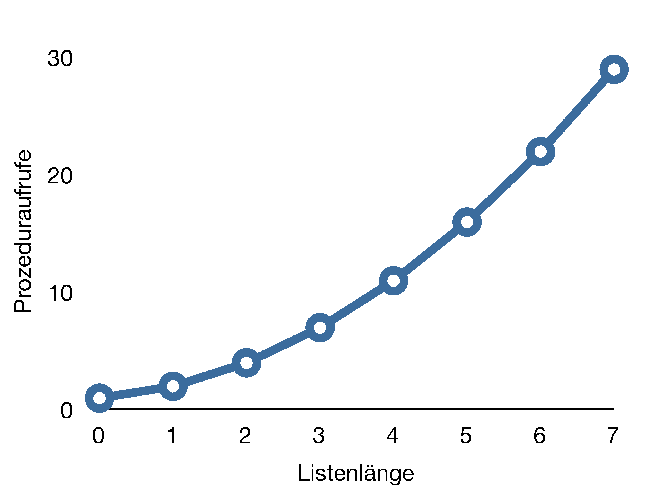
\includegraphics[width=0.5\textwidth]{invert-calls.eps}
  \caption{Funktionaufrufe bei \texttt{invert}}
  \label{fig:invert-calls}
\end{figure}
%
Doch zurück zu \texttt{invert}.  Obwohl die zu erledigende Aufgabe
einfach erscheint, dauert schon das Invertieren von Listen der Länge
1000 eine ganze Weile.\footnote{So war es zumindest zur Zeit der
  Drucklegung dieses Buchs auf handelsüblichen Computern.  Ggf.\
  müssen es auf moderneren Rechnern Listen der Länge 10000 sein, um
  das Problem deutlich zu machen.}  
Tatsächlich ist es so, daß z.B.\
das Invertieren einer Liste der Länge 400 \emph{mehr} als doppelt so
lang wie das Invertieren einer Liste der Länge 200 benötigt.  Das
liegt daran, daß \texttt{invert} bei jedem rekursiven Aufruf
\texttt{append-element} aufruft, und \texttt{append-element} selbst
macht soviele rekursive Aufrufe wie die Liste lang ist.  Das wiederum
heißt aber, daß die Gesamtanzahl der Funktionaufrufe für das
Invertieren einer Liste der Länge $n$ so steigt wie in
der Kurve in Abbildung~\ref{fig:invert-calls} gezeigt, also offenbar
stärker als linear: Das erklärt das überproportionale Ansteigen der
Rechenzeit.  (Dafür ist auch Aufgabe~\ref{ref:o-of-invert} relevant.)
Dies ist für so eine einfache Aufgabe
inakzeptabel: Listen der Länge 10000 sind nichts ungewöhnliches, und
das Invertieren sollte dem Computer leichtfallen.

Tatsächlich gibt es eine bessere Methode, eine Liste umzudrehen: Die
obige \texttt{invert}"=Funktion konstruiert die Ergebnisliste, indem
stets Elemente \emph{hinten} angehängt werden.  Das entspricht 
nicht der "`natürlichen"' Konstruktion von Listen mit
\texttt{make-pair}, das ein Element \emph{vorn} anhängt.  
Das Ergebnis ließe sich aber durch Anhängen vorn ganz einfach
konstruieren, und zwar, indem in folgender Reihenfolge
Zwischenergebnisse\index{Zwischenergebnis} berechnet werden, wie in folgendem Beispiel für den
Testfall \texttt{(invert (list 1 2 3 4))}:
%
\begin{verbatim}
#<empty-list>
#<list 1>
#<list 2 1>
#<list 3 2 1>
#<list 4 3 2 1>
\end{verbatim}
%
Jedes Zwischenergebnis entsteht aus dem vorhergehenden, indem ein
Element vorn an die Liste darüber angehängt wird.  Dies geschieht in
der Reihenfolge, in der die Elemente in der ursprünglichen Liste
auftreten: scheinbar einfach.  Allerdings erlaubt die normale
Konstruktionsanleitung für Listen nicht, dieses Zwischenergebnis
mitzuführen: Das Ergebnis des rekursiven Aufrufs \texttt{(invert (rest
  lis))} ist unabhängig vom Wert von \texttt{(first lis)}.  Damit aber
ist es der Funktion aus der normalen Konstruktionsanleitung unmöglich,
die obige Folge von Zwischenergebnissen nachzuvollziehen, da von einem
Zwischenergebnis zum nächsten gerade \texttt{(first lis)} vorn
angehängt wird.  Für diesen speziellen Fall~-- wenn eine Berechnung das
Mitführen von Zwischenergebnissen erfordert~-- muß die normale
Konstruktionsanleitung deshalb angepaßt werden.

Dieses Problem läßt sich durch Mitführen des Zwischenergebnisses in
einem separaten Parameter lösen, dem sogenannten
\textit{Akkumulator\index{Akkumulator}}.  Dazu wird eine
Hilfsfunktion \texttt{invert-helper} definiert, die neben der Eingabeliste
diesen Akkumulator akzeptiert:
%
\begin{verbatim}
(: invert-helper ((list-of %a) (list-of %a) -> (list-of %a)))

(define invert-helper
  (lambda (lis acc)
    ...))
\end{verbatim}
%
Die Liste \texttt{lis} ist nach wie vor die bestimmende Eingabe, es
greifen also die entsprechenden Konstruktionsanleitungen für gemischte
und zusammengesetzte Daten:
%
\begin{verbatim}
(define invert-helper
  (lambda (lis acc)
    (cond
      ((empty? lis) ...)
      ((pair? lis)
       ... (first lis) ...
       ... (invert-helper (rest lis) ...) ...))))
\end{verbatim}
%
Wenn \texttt{invert-helper} aufgerufen wird, sind die noch zu
verarbeitenden Elemente der ursprünglichen Liste in \texttt{lis}, und
das Zwischenergebnis, was aus den Elementen davor berechnet wurde, ist
in \texttt{acc}.  Wenn \texttt{lis} leer ist, sind alle Elemente
verarbeitet und das Zwischenergebnis ist das Endergebnis:
%
\begin{verbatim}
(define invert-helper
  (lambda (lis acc)
    (cond
      ((empty? lis) acc)
      ((pair? lis)
       ... (first lis) ...
       ... (invert-helper (rest lis) ...) ...))))
\end{verbatim}
%
Für den rekursiven Aufruf muß noch ein neuer Wert für \texttt{acc}
übergeben werden.  Dieser entsteht, wie im Beispiel zu sehen ist,
dadurch, daß an den Akkumulator das erste Element der Liste vorn
angehängt wird:
%
\begin{verbatim}
(define invert-helper
  (lambda (lis acc)
    (cond
      ((empty? lis) acc)
      ((pair? lis)
       ... (invert-helper (rest lis)
                          (make-pair (first lis) acc)) ...))))
\end{verbatim}
%
Da der rekursive Aufrufs von \texttt{invert-helper} schließlich direkt das
Endergebnis zurückgegeben wird, ist damit die Funktion auch schon fertig:
%
\begin{verbatim}
(define invert-helper
  (lambda (lis acc)
    (cond
      ((empty? lis) acc)
      ((pair? lis)
       (invert-helper (rest lis)
                      (make-pair (first lis) acc))))))
\end{verbatim}
%
Die neue Hilfsfunktion \texttt{invert-helper} paßt nicht auf die Signatur
von \texttt{invert}; \texttt{invert} muß also separat definiert werden
und den passenden Anfangswert für \texttt{acc} übergeben:
%
\begin{verbatim}
(define invert
  (lambda (lis)
    (invert-helper lis empty)))
\end{verbatim}
%
% Da \texttt{invert-helper} ausschließlich als Hilfsfunktion zu
% \texttt{invert} benutzt wird und ohne \texttt{invert} keinen Nutzen
% hat, ist es nicht notwendig, eine separate Signatur für
% \texttt{invert-helper} anzugeben. HK: Wir haben aber schon eine Signatur
% dafür angegeben! ;-)

Die neue Version von \texttt{invert} kommt ohne
\texttt{append-element} aus.  Der Beispielaufruf von oben führt zu
folgender Auswertung im Substitutionsmodell, die sich auch im Stepper
gut nachvollziehen läßt:
%
\begin{alltt}\small
(invert \underline{(list 1 2 3 4)})
\(\Longrightarrow\ldots\Longrightarrow\) (\underline{invert-helper} #<list 1 2 3 4> empty)
\(\Longrightarrow\ldots\Longrightarrow\) (cond ((empty? #<list 1 2 3 4>) ...) ((pair? #<list 1 2 3 4>) ...))
\(\Longrightarrow\ldots\Longrightarrow\) (invert-helper (rest #<list 1 2 3 4>) (make-pair (first #<list 1 2 3 4>) empty))
\(\Longrightarrow\ldots\Longrightarrow\) (invert-helper #<list 2 3 4> (make-pair 1 empty))
\(\Longrightarrow\ldots\Longrightarrow\) (invert-helper #<list 2 3 4> #<list 1>)
\(\Longrightarrow\ldots\Longrightarrow\) (cond ((empty? #<list 2 3 4>) ...) ((pair? #<list 2 3 4>) ...))
\(\Longrightarrow\ldots\Longrightarrow\) (invert-helper (rest #<list 2 3 4>) (make-pair (first #<list 2 3 4>) #<list 1>))
\(\Longrightarrow\ldots\Longrightarrow\) (invert-helper #<list 3 4> (make-pair 2 #<list 1>))
\(\Longrightarrow\ldots\Longrightarrow\) (invert-helper #<list 3 4> #<list 2 1>)
\(\Longrightarrow\ldots\Longrightarrow\) (cond ((empty? #<list 3 4>) ...) ((pair? #<list 3 4>) ...))
\(\Longrightarrow\ldots\Longrightarrow\) (invert-helper (rest #<list 3 4>) (make-pair (first #<list 3 4>) #<list 2 1>))
\(\Longrightarrow\ldots\Longrightarrow\) (invert-helper #<list 4> (make-pair 3 #<list 2 1>))
\(\Longrightarrow\ldots\Longrightarrow\) (invert-helper #<list 4> #<list 3 2 1>)
\(\Longrightarrow\ldots\Longrightarrow\) (cond ((empty? #<list 4>) ...) ((pair? #<list 4>) ...))
\(\Longrightarrow\ldots\Longrightarrow\) (invert-helper (rest #<list 4>) (make-pair (first #<list 4>) empty))
\(\Longrightarrow\ldots\Longrightarrow\) (invert-helper #<empty-list> (make-pair 4 #<list 3 2 1>))
\(\Longrightarrow\ldots\Longrightarrow\) (invert-helper #<empty-list> #<list 4 3 2 1>)
\(\Longrightarrow\ldots\Longrightarrow\) (cond ((empty? #<empty-list>) #<list 4 3 2 1>) ((pair? #<empty-list>) ...))
\(\Longrightarrow\) #<list 4 3 2 1>
\end{alltt}
%
Tatsächlich arbeitet die neue Funktion auch effizienter: Da
\texttt{invert-helper} nicht bei jedem Aufruf selbst wieder eine Funktion
aufruft, die eine komplette Liste verarbeitet, steigt die Rechenzeit
nur noch proportional zur Länge der Liste.

Da die Funktion \texttt{invert} generell nützlich ist, ist sie unter
dem Namen \texttt{reverse\index{reverse@\texttt{reverse}}} fest eingebaut.

\begin{feature}{\texttt{letrec}}{scheme:letrec}
Die \texttt{letrec}-Form bindet lokale Variablen, ähnlich wie \texttt{let}.
Ihre Syntax ist mit der von \texttt{let} identisch.  Während bei \texttt{let}
die Variablen, die an die Werte der Ausdrücke gebunden werden,
in den Ausdrücken selbst nicht sichtbar sind, sind bei \texttt{letrec}\index{letrec@\texttt{letrec}}
die Bindungen sichtbar.  
\end{feature}

Die Funktion \texttt{invert-helper} wird nur an einer einzigen Stelle
aufgerufen, und zwar innerhalb von \texttt{invert}. Es würde auch kaum einen
Sinn ergeben, \texttt{invert-helper} von einer anderen Stelle aus
aufzurufen. Deshalb bietet es sich an, für \texttt{invert-helper} eine lokale
Definition zu verwenden, die nur innerhalb von \texttt{invert} sichtbar
ist. Dazu gibt es im Prinzip die \texttt{let}-Form, die allerdings für
diesen Zweck nicht verwendbar ist (Abb.~\ref{scheme:letrec}). Die dort
vorgestellte \texttt{letrec}-Form löst das Problem.

Akkumulatoren, die Zwischenergebnisse verwalten, sind bei der Lösung
einer Reihe von Problemen nützlich.  Zum Beispiel könnte eine
Funktion, welche die Fakultät $n!$ einer Zahl $n$ berechnet,
vorgehen, indem sie das Produkt $n \cdot \ldots \cdot 1$ schrittweise von
links her ausrechnet:
%
\begin{displaymath}
  \xymatrix@R=10pt@C=2pt{
      &       &   & & 1\ar@{-->}[dllll]\\
    1 & \cdot & 4 &=& 4\ar@{-->}[dllll]\\
    4 & \cdot & 3 &=& 12\ar@{-->}[dllll]\\
    12 & \cdot & 2 &=& 24\ar@{-->}[dllll]\\
    24 & \cdot & 1 &=& 24\ar@{-->}[dllll]\\
    24
    }
\end{displaymath}
%
Der Anfangswert für das Zwischenergebnis ist 1, also gerade die
Fakultät von 0.

Für die Konstruktion wird die Schablone für Funktionen, die natürliche
Zahlen verarbeiten, um einen Akkumulator erweitert:
\label{page:factorial-tail}
%
\begin{verbatim}
; Fakultät berechnen

(: ! (natural -> natural))

(check-expect (! 0) 1)
(check-expect (! 3) 6)
(check-expect (! 5) 120)

(: ! (natural -> natural))
(define !
  (lambda (n)
    (letrec
        ((!-helper
          (lambda (n acc)
             (if (= n 0)
                acc
                ... ))))
      (!-helper n 1))))
\end{verbatim}
%
Wie aus der Beispielrechnung ersichtlich ist, wird aus dem "`alten"'
Zwischenergebnis das "`neue"' Zwischenergebnis, indem jeweils
mit \texttt{n} multipliziert wird:
%
\begin{verbatim}
    (letrec
        ((!-helper
          (lambda (n acc)
             (if (= n 0)
                acc
        ... (!-helper (- n 1) (* n acc)) ...))))
\end{verbatim}
%
Wie schon bei \texttt{invert} ist es nicht notwendig, daß für die
noch verbleibenden Ellipsen etwas eingesetzt wird; das Programm ist
bereits fertig:
%
\begin{verbatim}
(: ! (natural -> natural))
(define !
  (lambda (n)
    (letrec
        ((!-helper
          (lambda (n acc)
             (if (= n 0)
                acc
                (!-helper (- n 1) (* n acc)) ...))))
      (!-helper n 1))))
\end{verbatim}
%
Tatsächlich ist es bei Funktionen mit Akkumulator grundsätzlich nicht
notwendig, für die Ellipsen am Schluß etwas einzusetzen. Bei der
normalen Schablone für Funktionen, die Listen bzw.\ natürliche Zahlen
verarbeiten, wird für diese Ellipsen Code eingesetzt, was das erste
Element der Liste mit dem Ergebnis des rekursiven Ausdrucks 
zum Rückgabewert kombiniert.  Dies ist beim Einsatz eines Akkumulators
aber nicht notwendig, da das erste Element der Liste bereits in die
Berechnung des nächsten Zwischenergebnisses eingeht und dieses
Zwischenergebnis beim letzten Aufruf bereits das Endergebnis ist.

\section{Schablonen für Funktionen mit Akkumulator}

Aus den beiden Beispielen des vorgehenden Abschnitts ergeben sich
direkt Schablonen für Funktionen mit Akkumulator.  Zunächst die
Schablone für Funktionen mit Akkumulator, die Listen akzeptieren:
%
\begin{alltt}
(: proc ((list-of elem) -> ...))

(define proc
  (lambda (lis)
    (letrec
       ((proc-helper
         (lambda (lis acc)
            (cond
              ((empty? lis) acc)
              ((pair? lis)
                 (proc-helper (rest lis)
                    (... (first lis) ... acc ...)))))))
    (proc-helper lis z))))
\end{alltt}
%
Hier ist \texttt{proc} der Name der zu definierenden Funktion
und \texttt{proc-helper} der Name der Hilfsfunktion mit
Akkumulator.  Der Anfangswert für den Akkumulator~-- also das initiale
Zwischenergebnis~-- ist der Wert von \texttt{z}.  Der
Ausdruck, der für \texttt{(... (first lis) ... acc ...)} einzusetzen
ist, macht aus dem alten Zwischenergebnis \texttt{acc} das neue
Zwischenergebnis.

Die Schablone für Funktionen mit Akkumulator, die natürliche Zahlen
akzeptieren, ist analog:
%
\begin{alltt}
(: proc (natural -> ...))

(define proc
  (lambda (n)
    (letrec
      ((proc-helper
        (lambda (n acc)
          (if (= n 0)
              acc
              (proc-helper (- n 1) (... acc ...))))))
    (proc-helper n z))))
\end{alltt}
%
Wieder ist \texttt{z} der Ausdruck für das initiale Zwischenergebnis
und für \texttt{(... acc ...)} ist ein Ausdruck einzusetzen, der aus
dem alten Zwischenergebnis \texttt{acc} ein neues macht.

\section{Kontext und Endrekursion}
\label{sec:iteration}

Ein Vergleich der beiden Versionen der Fakultätsfunktion von
S.~\pageref{page:factorial} und S.~\pageref{page:factorial-tail} zeigt, daß
Formulierungen mit und ohne Akkumulator
unterschiedliche Berechnungsprozesse erzeugen.  Hier ein Prozeß mit
Akkumulator:
%
\begin{alltt}
(! 4)
\(\Longrightarrow\) (!-helper 4 1)
\(\Longrightarrow\) (if (= 4 0) 1 (!-helper (- 4 1) (* 1 4)))
\(\Longrightarrow\) (if #f 1 (!-helper (- 4 1) (* 1 4)))
\(\Longrightarrow\) (!-helper (- 4 1) (* 1 4))
\(\Longrightarrow\) (!-helper 3 4)
\(\Longrightarrow\) (if (= 3 0) 4 (!-helper (- 3 1) (* 4 3)))
\(\Longrightarrow\) (if #f 4 (!-helper (- 3 1) (* 4 3)))
\(\Longrightarrow\) (!-helper (- 3 1) (* 4 3))
\(\Longrightarrow\) (!-helper 2 12)
\(\Longrightarrow\) (if (= 2 0) 12 (!-helper (- 2 1) (* 12 2)))
\(\Longrightarrow\) (if #f 12 (!-helper (- 2 1) (* 12 2)))
\(\Longrightarrow\) (!-helper (- 2 1) (* 12 2))
\(\Longrightarrow\) (!-helper 1 24)
\(\Longrightarrow\) (if (= 1 0) 24 (!-helper (- 1 1) (* 24 1)))
\(\Longrightarrow\) (if #f 24 (!-helper (- 1 1) (* 24 1)))
\(\Longrightarrow\) (!-helper (- 1 1) (* 1 24))
\(\Longrightarrow\) (!-helper 0 24)
\(\Longrightarrow\) (if (= 0 0) 24 (!-helper (- 0 1) (* 24 0)))
\(\Longrightarrow\) (if #t 24 (!-helper (- 0 1) (* 24 0)))
\(\Longrightarrow\) 24
\end{alltt}
%
Demgegenüber hier der Prozeß ohne Akkumulator:
%
\begin{alltt}
(! 4)
\(\Longrightarrow\) (if (= 4 0) 1 (* 4 (! (- 4 1))))
\(\Longrightarrow\) (if #f 1 (* 4 (! (- 4 1))))
\(\Longrightarrow\) (* 4 (! (- 4 1)))
\(\Longrightarrow\) (* 4 (! 3))
\(\Longrightarrow\) (* 4 (if (= 3 0) 1 (* 3 (! (- 3 1)))))
\(\Longrightarrow\) (* 4 (if #f 1 (* 3 (! (- 3 1)))))
\(\Longrightarrow\) (* 4 (* 3 (! (- 3 1))))
\(\Longrightarrow\) (* 4 (* 3 (! 2)))
\(\ldots\)
\(\Longrightarrow\) (* 4 (* 3 (* 2 (! 1))))
\(\Longrightarrow\) (* 4 (* 3 (* 2 (if (= 1 0) 1 (* 1 (! (- 1 1)))))))
\(\Longrightarrow\) (* 4 (* 3 (* 2 (if #f ... (* 1 (! (- 1 1)))))))
\(\Longrightarrow\) (* 4 (* 3 (* 2 (* 1 (! (- 1 1))))))
\(\Longrightarrow\) (* 4 (* 3 (* 2 (* 1 (! 0)))))
\(\Longrightarrow\) (* 4 (* 3 (* 2 (* 1 (if (= 0 0) 1 (* 0 (! (- 0 1))))))))
\(\Longrightarrow\) (* 4 (* 3 (* 2 (* 1 (if #t 1 (* 0 (! (- 0 1)))))))))
\(\Longrightarrow\) (* 4 (* 3 (* 2 (* 1 1))))
\(\Longrightarrow\) (* 4 (* 3 (* 2 1)))
\(\Longrightarrow\) (* 4 (* 3 2))
\(\Longrightarrow\) (* 4 6)
\(\Longrightarrow\) 24
\end{alltt}
%
Es ist deutlich sichtbar, daß die Version ohne Akkumulator alle
Multiplikationen bis zum Schluß "`aufstaut"'.  Das heißt aber auch,
daß im Laufe des Berechnungsprozesses Ausdrücke auftauchen, die desto
größer werden je größer das Argument von \texttt{!} ist: Bei
\texttt{(!  100)} werden zum Beispiel 100 Multiplikationen aufgestaut.

Die Version mit Akkumulator hingegen scheint in der Größe der
zwischenzeitlich auftretenden Ausdrücke begrenzt zu sein.  Tatsächlich
stellt sich das Wachstum der Version ohne Akkumulator bei der Version
mit Akkumulator nicht ein.

Der Grund dafür sind die Schablonen: In der Schablone für Funktionen
ohne Akkumulator steht \texttt{(... (proc (- n 1)) ...)}, das
heißt, um den rekursiven Aufruf von \texttt{proc} wird noch
etwas "`herumgewickelt"', oder, anders gesagt, mit dem Ergebnis des
rekursiven Aufrufs passiert noch etwas.  Das, was mit dem Ergebnis
noch passiert, heißt der \textit{Kontext\index{Kontext}} des Aufrufs.
Bei \texttt{!} ist der vollständige Ausdruck \texttt{(* n (! (- n
  1)))}.  Wenn aus diesem Ausdruck der rekursive Aufruf \texttt{(! (-
  n 1))} herausgenommen wird, bleibt der Kontext \texttt{(* n
  \(\circ\))}, wobei $\circ$ markiert, wo der Aufruf entfernt
wurde.  Tatsächlich wird in der Literatur diese Markierung
\textit{Loch\index{Loch}} genannt und \texttt{[]} geschrieben.  Der
Kontext \texttt{(* n [])} macht deutlich, daß mit Ergebnis eines
Aufrufs, der später für \texttt{[]} eingesetzt wird, noch \texttt{n}
multipliziert wird.  Dementsprechend stauen sich in der
Reduktionsfolge die Multiplikationen mit den verschiedenen Werten von
\texttt{n}.

Bei der Fakultäts-Funktion mit Akkumulator ist der Ausdruck, zu dem
der Rumpf bei $\texttt{n} \neq 0$ reduziert wird, \texttt{(!-helper (- n 1)
  (* n acc))}.  Der Kontext des Aufrufs von \texttt{!-helper} innerhalb
dieses Ausdrucks ist \texttt{[]}, also \emph{leer}~-- \emph{nichts}
passiert mehr mit dem Rückgabewert von \texttt{!-helper}, und damit stauen
sich auch bei der Reduktion keine Kontexte an.  Solche Funktionaufrufe
ohne Kontext heißen \textit{endrekursiv\index{endrekursiv}}~-- eben,
weil nach dem rekursiven Aufruf "`Ende"' ist.\footnote{Das Konzept des
  Aufrufs ohne Kontext ist nicht auf rekursive Aufrufe beschränkt.  Im
  Englischen heißen solche Aufrufe allgemeiner \textit{tail
    calls\index{tail call}} (also ohne "`recursive"').}
Die Berechnungsprozesse, die von endrekursiven Aufrufen generiert
werden, heißen auch \textit{iterative\index{Iteration}} Prozesse.

\section{Das Phänomen der umgedrehten Liste}

Die beiden Varianten der Fakultäts-Funktion berechnen zwar beide 
stets das gleiche Ergebnis.  Die beiden Reduktionsfolgen für
\texttt{(! 4)} aus dem vorigen Abschnitt zeigen allerdings, daß die
beiden Funktionen bei der Berechnung unterschiedlich vorgehen:
Während die Variante ohne Akkumulator "`von rechts"' multipliziert,
also folgendermaßen auswertet:
%
\begin{displaymath}
  4\cdot (3 \cdot (2 \cdot (1 \cdot 1)))
\end{displaymath}
%
multipliziert die Variante mit Akkumulator "`von links"':
%
\begin{displaymath}
  (((1 \cdot 4)\cdot 3)\cdot 2)\cdot 1
\end{displaymath}
%
Die Multiplikationen passieren also in umgekehrter Reihenfolge.
Dies macht bei der Fakultät keinen Unterschied, da die Multiplikation
assoziativ ist.  Diese Assoziativität ist jedoch nicht immer
gegeben~-- insbesondere nicht bei Funktionen, die Listen zurückgeben.
Hier zum Beispiel eine Funktion, die eine Zahl $n$ akzeptiert und eine
absteigende Liste der Zahlen von $n$ bis $1$ zurückliefert:
%
\begin{verbatim}
; Liste der Zahlen von n bis 1 generieren
(: build-list (natural -> (list-of natural)))

(check-expect (build-list 0) empty)
(check-expect (build-list 3) (list 3 2 1))

(define build-list
  (lambda (n)
    (if (= n 0)
        empty
        (make-pair n (build-list (- n 1))))))
\end{verbatim}
%
Die direkte Übersetzung in eine Variante mit Akkumulator liefert:
%
\begin{verbatim}
(define build-list
  (lambda (n)
    (letrec
      ((build-list-helper
        (lambda (n acc)
          (if (= n 0)
              acc
              (build-list-helper (- n 1) (make-pair n acc))))))
    (build-list-helper n empty))))
\end{verbatim}
%
Diese Variante ist inkorrekt: Sie liefert z.B.\ für
\texttt{(build-list 3)} das Ergebnis \verb|#<list 1 2 3>|, die
Elemente der Liste sind also in umgekehrter Reihenfolge.  Da schon die
Fakultätsfunktion mit Akkumulator die Multiplikationen gegenüber der
Variante ohne Akkumulator in umgekehrter Reihenfolge durchgeführt hat, war dies allerdings zu
erwarten, und ist ein generelles Phänomen bei der Berechnung von
Listen-Ausgaben mit Akkumulator.  Das Problem kann durch das Umdrehen
der Ergebnisliste gelöst werden:
%
\begin{verbatim}
    (letrec
      ((build-list-helper
        (lambda (n acc)
          (if (= n 0)
              (reverse acc)
              (build-list-helper (- n 1) (make-pair n acc))))))
\end{verbatim}
%


\section*{Anmerkungen}

Bei der Auswertung von Programmen durch den Computer wird für die
Verwaltung von Kontexten Speicherplatz benötigt: Bei rekursiven
Funktionen ohne Akkumulator wächst dieser Speicherplatz mit der Größe
der Argumente.  Entsprechend wird prinzipiell kein Speicherplatz
benötigt, wenn kein Kontext anfällt.  In den Lehrsprachen  wird auch tatsächlich
kein Speicherplatz für endrekursive Aufrufe verbraucht; dies ist
allerdings bei vielen anderen Programmiersprachen nicht der Fall.
Mehr dazu in Kapitel~\ref{cha:secd}.

\section*{Aufgaben}

\begin{aufgabe}
  \label{ref:o-of-invert}
  Entwicklen Sie eine Formel für die Anzahl der rekursiven Aufrufe in
  der ersten Version von \texttt{invert}!  (Hinweis: Greifen Sie auf
  die Gauß'sche Summenformel zurück.)
\end{aufgabe}

\begin{aufgabe}
  Schreiben Sie eine Funktion \texttt{list-sum+product}, die eine
  Liste von Zahlen akzeptiert und eine zweielementige Liste
  zurückgibt, deren erstes Element die Summe der Listenelemente und
  deren zweites Element ihr Produkt ist.  Schreiben Sie zwei Varianten
  der Funktion: eine ohne Akkumulator und eine mit zwei Akkumulatoren.
\end{aufgabe}

\begin{aufgabe}
  Schreiben Sie eine Funktion, die als Eingabe eine Liste von Kursen
  einer Aktie (als Zahlen) eines Tages akzeptiert (nach Tageszeit
  aufsteigend sortiert), und als Rückgabewert den höchstmöglichen
  Gewinn liefert, die durch den Kauf und folgenden Verkauf der Aktie
  an diesem Tag erreicht werden kann.

  Hinweis: Diese Funktion benötigt zwei Akkumulatoren.
\end{aufgabe}

\begin{aufgabe}
  Schreibe zu der Funktion \texttt{power} aus Aufgabe~\ref{aufg:power} eine
  endrekursive Variante.
\end{aufgabe}

\begin{aufgabe}
  Identifizieren Sie die Kontexte der Aufrufe der Funktionen namens
  \texttt{p} in folgenden Ausdrücken:
  
\begin{verbatim}
(+ (p (- n 1)) 1)
(p (- n 1) acc)
(* (p (rest lis)) b)
(+ (* 2 (p (- n 1))) 1)
(p (- n 1) (* acc n))
(f (p n))
(+ (f (p n)) 5)
(p (f (- n 1)) (* n (h n))) 
(+ (f (p n)) (h n))
\end{verbatim}
  %
  Welche Aufrufe sind endrekursiv bzw.\ \textit{tail calls}?
\end{aufgabe}

\begin{aufgabe}
  Schreibe eine endrekursive Variante von \texttt{list-length}.
\end{aufgabe}

\begin{aufgabe}
  Schreibe eine endrekursive Variante von
  \texttt{concatenate}.  Falls du Hilfsfunktionen auf
  Listen dafür benutzt, gib auch dafür endrekursive Definitionen an.
\end{aufgabe}

\begin{aufgabe}
  Schreibe endrekursive Varianten von \texttt{evens} und \texttt{odds}
  aus Aufgabe~\ref{ex:evensodds} auf Seite~\pageref{ex:evensodds}.
  Falls du Hilfsfunktionen auf Listen dafür benutzt, gib auch dafür
  endrekursive Definitionen an.
\end{aufgabe}

\begin{aufgabe}
  Schreiben Sie eine endrekursive Variante von \texttt{power} aus
  Aufgabe~\ref{aufg:power} von Seite~\pageref{aufg:power}.
\end{aufgabe}

%%% Local Variables: 
%%% mode: latex
%%% TeX-master: "i1"
%%% End: 

